\subsection{Elektroninė metalų laidumo teorija}

Metaluose krūvio nešėjai yra elektronai. Pagrindimas: 

Elektronas, susidūręs su metalo gardelės jonu, gali pradėti judėti
bet kuria kryptimi ir po kiekvieno tokio susidūrimo dreifuojančio
elektrono pradinis greitis yra lygus nuliui. Dėl elektrinio lauko
poveikio, elektronas pradeda judėti jo veikimo kryptimi ir per laiką
$t$ vėl sutinka gardelės joną.

Elektrono inercijos jėga:
\begin{equation*}
  F_{\t{in}} = -ma
\end{equation*}
čia:
\begin{description}
  \item[$m$] – masė;
  \item[$a$] – pagreitis.
\end{description}

Elektros šaltinio kuriama elektros varomoji jėga:
\begin{align}
  E &= \frac{A_{\t{paš}}}{q} \\
  \intertext{Kadangi darbas yra lygus jėgos ir kelio sandaugai:}
  &= \frac{F_{\t{in}} l}{q} \\
  &= -\frac{mal}{q} \\
  \intertext{Pagal apibrėžimą, pagreitis yra greičio pokytis per laiko
  vienetą. Kadangi, pas mus pradinis greitis yra 0, tai gauname:}
  &= -\frac{mvl}{qt} \label{eq:metalu_laidumo_1} \\
\end{align}
čia:
\begin{description}
  \item[$A_{\t{paš}}$] – pašalinių jėgų darbas;
  \item[$q$] – pratekėjęs krūvis;
  \item[$F_{\t{in}}$] – inercijos jėga;
  \item[$l$] – laidininko ilgis.
  \item[$v$] – elektrono per laiką $t$ pasiektas greitis;
  \item[$t$] – po kiek laiko nuo judėjimo pradžios elektronas sutiko
    joną.
\end{description}

Krūvis, kuris prateka laidininku:
\begin{equation}
  Q = I t \label{eq:metalu_laidumo_3}
\end{equation}
čia:
\begin{description}
  \item[$I$] – srovės stipris.
\end{description}

Iš Omo dėsnio:
\begin{align}
  I &= \frac{E}{R} \\
  \intertext{Įsistatome \ref{eq:metalu_laidumo_1} ir gauname:}
  &= -\frac{mal}{Rq} \label{eq:metalu_laidumo_2} \\
\end{align}
čia:
\begin{description}
  \item[$R$] – laidininkų ir galvanometro varža.
\end{description}

Sulyginę \ref{eq:metalu_laidumo_2} ir \ref{eq:metalu_laidumo_3}
gauname:
\begin{align*}
  I &= \frac{mlv_{0}}{qRt} \\
  &= \frac{Q}{t} \\
  \frac{q}{m}
  &= \frac{v_{0}l}{QR} \\
  &= (\t{nuo }1,5 \t{ iki } 1,6) \cdot 10^{11} \tfrac{C}{kg}
\end{align*}
čia:
\begin{description}
  \item[$\frac{q}{m}$] – savitasis dalelės krūvis.
\end{description}

Gautąjį savitąjį dalelės krūvį palyginę su elektrono:
\begin{align*}
  \frac{e}{m} &= 1,76 \cdot 10^{11} \tfrac{C}{kg}.
\end{align*}
galime teigti, jog krūvio nešėjai yra elektronai.

TODO: Suprasti ir perrašyti.

\begin{align*}
  \frac{mv^{2}}{2} &= \frac{3}{2} k T
\end{align*}

\begin{align*}
  v_{kv} &= 1,1 \cdot 10^{5} \tfrac{m}{s}
\end{align*}

Tvarkingo judėjimo greitis:
\begin{align*}
  v &\equiv 8 \cdot 10^{-4} \tfrac{m}{s}
\end{align*}

Vidutinis elektrono greitis (?):
\begin{align*}
  \t{ū} &= 10^{6} \tfrac{m}{s}
\end{align*}

Elektrono greitis:
\begin{align*}
  v &= \mu E
\end{align*}

\section{Magnetinis laukas}

\subsection{Srovės magnetinis laukas}

Kol laidininke srovė neteka, magnetinė rodyklė nusistovi pagal Žemės
magnetinio lauko kryptį. Kai srovė teka – rodyklė stengiasi pasisukti
statmenai laidininkui – ją veikia srovės magnetinis laukas. Tai nustatė
Erstedas 1820 metais. Kadangi srovė laidininke yra tvarkingas elektronų
judėjimas, tai reiškia, kad apie bet kokį judantį krūvį turi egzistuoti
magnetinis laukas.

\begin{defn}[Magnetinis laukas]
  Ypatingos formos materija, perduodanti judančių elektros krūvių
  sąveiką.
\end{defn}

\begin{defn}[Magnetinio lauko stipris]
  Dydis apibūdinantis magnetinio lauko stiprumą vakuume.
  \begin{equation*}
    H = \frac{I}{l}
  \end{equation*}
  čia:
  \begin{description}
    \item[$\vec{H}$] – magnetinio lauko stipris (matuojamas $\frac{A}{m}$);
    \item[$I$] – srovės stipris;
    \item[$l$] – magnetinės linijos, einančios per duotąjį tašką, ilgis.
  \end{description}
  Magnetinio lauko stiprio vektoriaus kryptis yra išilgai magnetinio
  lauko jėgų linijos liestinės į tą pusę, kurią rodo magnetinės rodyklės
  šiaurės polius.
\end{defn}

\begin{defn}[Magnetinė indukcija]
  Jėginė magnetininio lauko charakteristika. Apibūdina magnetinio lauko
  stiprumą medžiagoje.
  \begin{equation*}
    \vec{B} = \mu_{0} \mu \vec{H}
  \end{equation*}
  čia:
  \begin{description}
    \item[$\vec{B}$] – magnetinė indukcija (matuojama teslomis
      $1T = 1\frac{N}{Am}$);
    \item[$\mu_{0}$] – magnetinė konstanta 
      ($\mu_{0} = 4\pi \cdot 10^{-7} \frac{N}{A^{2}} = 1,25 \cdot 10^{-6} 
      \frac{N}{A^{2}}$);
    \item[$\mu$] – santykinė aplinkos magnetinė skvarba;
    \item[$\vec{H}$] – magnetinio lauko stipris.
  \end{description}
  Magnetinės indukcijos linijos apie laidininką, kuriuo teka srovė, yra
  išsidėsčiusios pagal dešiniojo sraigto taisyklę.
\end{defn}

\begin{defn}[Lorenco jėga]
  Jėga, kuria magnetinis laukas veikia judančią elektringąją dalelę:
  \begin{align*}
    F_{L}
    &= q | \vec{v} \cdot \vec{B}| \\
    &= q v B \sin \alpha \\
  \end{align*}
  čia:
  \begin{description}
    \item[$q$] – dalelės krūvis;
    \item[$\vec{v}$] – dalelės greitis;
    \item[$\vec{B}$] – magnetinės indukcijos vektorius;
    \item[$\alpha$] – kampas tarp $\vec{v}$ ir $\vec{B}$.
  \end{description}
  Lorenco jėga yra statmena $\vec{v}$ ir $\vec{B}$.
  (Žr. \ref{fig:lorenco_jega} paveikslėlį.)
\end{defn}

\begin{figure}[H]
  \begin{center}
    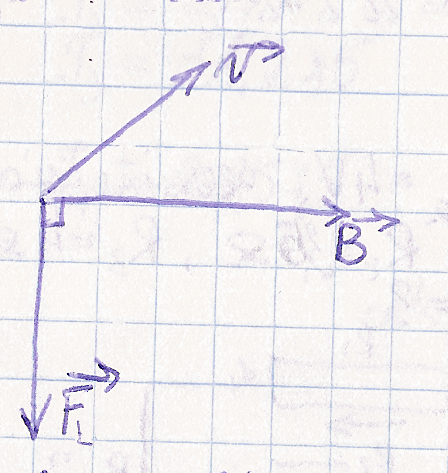
\includegraphics[height=0.5\textwidth]{images/lorenco_jega.png}
  \end{center}
  \caption{Lorenco jėga}
  \label{fig:lorenco_jega}
\end{figure}

\begin{defn}[Ampero jėga]
  Laidininką, kuriuo teka elektros srovė, magnetiniame lauke veikianti
  jėga.

  \begin{equation*}
    F_{A} = I l B \sin \alpha
  \end{equation*}
  čia:
  \begin{description}
    \item[$I$] – laidininku tekančios srovės stipris;
    \item[$l$] – laidininko ilgis;
    \item[$B$] – magnetinė indukcija;
    \item[$\alpha$] – kampas tarp elektros srovės ir magnetinės
      indukcijos krypčių.
  \end{description}
\end{defn}

\begin{note}
  Ampero jėgos išraišką galime nesunkiai gauti iš Lorenco jėgos
  išraiškos:
  \begin{align*}
    F
    &= q v B \sin \alpha \\
    &= \underbrace{I t}_{q} v B \sin \alpha \\
    &= I \underbrace{t v}_{l} B \sin \alpha \\
    &= I l B \sin \alpha \\
  \end{align*}
\end{note}

Elektromagnetiniame lauke judantį krūvį veikianti jėga:
\begin{align*}
  F &= q \vec{E} + q \left[ \vec{v} \cdot \vec{B} \right]
\end{align*}

\begin{defn}[Bio Savaro Laplaso dėsnis]
  Bet kurios srovės magnetinio lauko indukcija gali būti apskaičiuota,
  kaip magnetinių laukų, sukuriamų atskirų elementarių srovės
  elementų $d\vec{l}$, indukcijų vektorinė suma:
  \begin{align}
    d \vec{B} &=
      \frac{\mu_{0}}{4 \pi}
      \frac{I \left[ d\vec{l}, \vec{r} \right] }{r^{3}} \\
    dB &=
      \frac{\mu_{0}}{4\pi}\frac{I \cdot dl \cdot \sin \alpha}{r^{2}} 
      \label{eq:bsl_sin} \\
    \vec{B} &=
      \frac{\mu_{0}I}{4\pi}
      \int _{(l)} \frac{\left[ d\vec{l} \cdot \vec{r} \right]}{r^{3}} \\
  \end{align}
  čia:
  TODO: Paaiškinti. Šis dėsnis išvedamas iš:
  \begin{align*}
    \intertext{atskiras magnetinės jėgos tarp dviejų judančių
    krūvių atvejis:}
    F_{m} &= \frac{\mu_{0}q_{1}q_{2}v^{2}}{4\pi r^{2}} \\
    \intertext{bendras magnetinės jėgos tarp dviejų judančių krūvių
    atvejis:}
    \vec{F_{m}} &=
      \frac{\mu_{0} q_{1} q_{2}
        \left( \vec{v}_{2} \times (\vec{v_{1} \times \vec{r}}) \right)
        }{4 \pi r^{3}} \\
    \intertext{$\vec{v_{1}}$ greičiu judantis $q_{1}$ krūvis atstumu
      $\vec{r}$ kuria magnetinį lauką:}
      \vec{B} &=
        \frac{\mu_{0} q_{1} \left( \vec{v_{1}} \times \vec{r} \right)
        }{4 \pi r^{3}}
    \intertext{Atkarpėlės ilgį pažymėkime $dl$, o ja tekančios
    srovės stiprį $I$. Čia $|d\vec{l}| = dl$, o $d\vec{l}$ kryptis
    sutampa su srovės tekėjimo kryptimi. Krūvininkų skaičių srovės
    elemente pažymėkime $d N$, o jų dreifo greitį $v$, srovės elemento
    skerspjūvio plotą $S$, krūvininkų tankį $n$. Tada pasinaudodami
    (TODO: nuoroda), apskaičiuojame, kad srovės elemento sukurtas
    magnetinio srauto tankis:}
    d \vec{B} &=
      \frac{\mu_{0}q\left( \vec{v} \times \vec{r} \right)}{4 \pi r^3 }
      \cdot d N \\
    \intertext{Kadangi:}
    v &= \frac{I}{qnS} \\
    dN
    &= ndV \\
    &= n S dl \\
    \intertext{Gauname:}
    d \vec{B} &=
      \frac{\mu_{0}I\left( d \vec{l} \times \vec{r} \right)}{4 \pi r^3}
  \end{align*}
\end{defn}

\begin{exmp}
  Apskaičiuokime magnetinę indukciją $B$, kurią sukuria tiesus, plonas,
  be galo ilgas laidininkas atstumu $r_{0}$ nuo laido:
  \begin{align*}
    \intertext{nykstamai trumpos laidininko atkarpos kuriama magnetinė
    indukcija:}  
    B
    &= \mu_{0} \mu H \\
    &= \mu_{0} \mu \frac{I}{l} \\
    \intertext{$l$ yra apskritimo, kurio spindulys jungia tašką su 
    nagrinėjama laidininko atkarpa, ilgis:}
    l
    &= 2 \pi r \\
    &= 2 \pi \frac{r_{0}}{\cos \alpha} \\
    \intertext{sujungę gauname:}
    B
    &= \mu_{0} \mu \frac{I \cos \alpha}{2 \pi r_{0}} \\
    \intertext{kadangi mūsų laidininkas yra begalinio ilgio, tai
    $\alpha$ kitimo sritis yra nuo $-\frac{\pi}{2}$ iki $\frac{\pi}{2}$:}
    B
    &= 2 \int _{0} ^{\frac{\pi}{2}} \mu_{0} \mu 
      \frac{I \cos \alpha}{2 \pi r_{0}} d \alpha \\
    &= 2 \mu_{0} \mu \frac{I}{2 \pi r_{0}}
      \int _{0} ^{\frac{\pi}{2}} \cos \alpha d\alpha \\
    &= \frac{\mu_{0} \mu}{\pi} \frac{I}{r_{0}}\\
    \intertext{FIXME: Turėjo gautis:}
    B &= \frac{\mu_{0} \mu}{2 \pi} \frac{I}{r_{0}}
  \end{align*}
\end{exmp}

\begin{exmp}
  \emph{Sąlyga.} Elektronas, kurio greitis yra $2 \cdot 10^{6} m/s$,
  įlekia į magnetinį lauką, kurio magnetinė indukcija $B = 0,03T$,
  kampu lygiu $\frac{\pi}{6}$. Rasti elektrono orbitos spindulį $r$
  ir poslinkį $h$ padarytą per vieną apsisukimą.

  Duota:
  \begin{align*}
    \alpha &= \frac{\pi}{6} \\
    B &= 0,03 T \\
    v_{0} &= 2 \cdot 10^{6} m/s \\
    e &= 1,6021773 \cdot 10^{-19} \\
    m_{e} &= 9,1093898 \cdot 10^{-31} \\
  \end{align*}

  TODO: Brėžinys. Tarkime, kad x ašis yra nukreipta magnetinio lauko
  linijų kryptimi ir elektrono pradinio greičio vektorius $\vec{v_{0}}$
  priklauso plokštumai $xOy$.

  Elektrono pradinis greitis susideda iš dviejų dedamųjų: $v_{0x}$ –
  greičio išilgai magnetinio lauko linijų ir greičio $v_{0y}$ –
  statmeno magnetinio lauko linijoms. Krūvio judančio išilgai
  magnetinio lauko linijų, magnetinės jėgos neveikia, taigi elektrono
  greičio $v_{x}$ dedamoji yra konstanta ir ji yra lygi $v_{0x}$.
  Krūvį judantį statmenai magnetinio lauko linijoms veikia jėga,
  kuri verčia krūvį suktis, o jos stiprumas yra lygus:
  \begin{align*}
    F
      &= B e v_{0y} \\
      &= B e v_{0} \sin \alpha. \\
    \intertext{Iš antro Niutono dėsnio žinome, kad}
    F
      &= ma. \\
    \intertext{Taip pat žinome, kad apskritimine trajektorija
    skriejančio kūno pagreitį, greitį ir trajektorijos spindulį
    sieja lygybė:}
    a
      &= \frac{v_{0y}^{2}}{r} \\
      &= \frac{(v_{0} \sin \alpha)^{2}}{r}. \\
    \intertext{Iš turimų formulių išsireiškiame $r$:}
    ma
      &= B e v_{0} \sin \alpha \\
    m \frac{(v_{0} \sin \alpha)^{2}}{r}
      &= B e v_{0} \sin \alpha \\
    m \frac{v_{0} \sin \alpha}{r}
      &= B e \\
    r
      &= \frac{m v_{0} \sin \alpha}{B e} \\
      &\approx 0,00018952 m. \\
    \intertext{Elektronas vieną kartą apsisuks per:}
    T
      &= \frac{2 \pi r}{v_{0y}} \\
    \intertext{Ir per tą laiką nuskries:}
    h
      &= v_{0x} T \\
      &= v_{0} \cos \alpha \frac{2 \pi r}{v_{0} \sin \alpha} \\
      &= \frac{2 \pi v_{0} m \cos \alpha}{Be} \\
      &\approx 0,00206251 m.
  \end{align*}

\end{exmp}

\begin{exmp}
  \emph{Sąlyga.} Protonas įlekia į magnetinį lauką greičiu
  $v (v = 10^{4}m/s)$. Indukcija $B = 0,01 T$. Kampas tarp vektorių
  $\vec{v}$ ir $\vec{B}$ yra $\frac{\pi}{3}$. Rasti protono judėjimo
  trajektoriją ($r$ ir $h$) ir kelią nueitą per 10 mikrosekundžių.

  Duota:
  \begin{align*}
    \alpha &= \frac{\pi}{3} \\
    B &= 0,01 T \\
    v_{0} &= 10^{4} m/s \\
    q &= 1,6021773 \cdot 10^{-19} \\
    m &= 1,6 \cdot 10^{-27} kg \\
    t &= 10^{-5} s \\
  \end{align*}

  Analogiškai praeitam uždaviniui:
  \begin{align*}
    r &= \frac{m v_{0} \sin \alpha}{B e} \\
    h &= \frac{2 \pi v_{0} m \cos \alpha}{Be} \\
    l &= v \cdot t \\
      &= 10^{4} \cdot 10^{-5} \\
      &= 0,1 m.\\
  \end{align*}

\end{exmp}
